The algorithms were implemented in C++. \textit{NetworKit} and \textit{Boost} frameworks were used for data structures (e.g. graph) and algorithms (e.g. for random graph generation and finding maximum matching). The implementation's source code was added to the \textbf{koala-networkit} repository and is available at \href{https://github.com/krzysztof-turowski/koala-networkit/pull/8}{\texttt{https://github.com/krzysztof-turowski/koala-networkit/pull/8}}. Classes BranchAndReduceMDS$\langle$GrandoniMSC$\rangle$, BranchAndReduceMDS$\langle$FominGrandoniKratschMSC$\rangle$, BranchAndReduceMDS$\langle$RooijBodlaenderMSC$\rangle$, FominKratschWoegingerMDS, SchiermeyerMDS implement algorithms of GRANDONI, Fomin-Grandoni-Kratsch, van Rooij-Bodlaender, Fomin-Kratsch-Woeginger, Schiermeyer, respectively.
\section{Implementation decisions}
\subsection{Measure and Conquer algorithms}
\begin{enumerate}
    \item Due to the fact that implementation is expected to run on instances that contain several dozen vertices, the asymptotic time of execution is not the only factor one should take care of. To enhance implementation's running time, one may consider avoiding some operations that are slow in practice. For instance, copying and allocating memory for the structures defining the correspondence of elements belonging to the sets. The alternative is to modify the structures before each call to the sub-problem and retrieve them whenever it returns.
    \item The family of sets in the sub-problems does not contain empty sets. These, however, may be present in memory representations of the structures used. They are not counted into the solution's cardinality and do not influence any high-level logic of the algorithm. 
\end{enumerate}
\subsection{Algorithms for the minimum optional dominating set}
\begin{enumerate}
    \item Similarly as for measure and conquer copying structures used in recursive calls are avoided, instead, these are modified and then restored properly after a recursive call.
    \item In the parts of the algorithms, where small dominating set candidates are tested (of cardinality up to $\frac{1}{3}|V(G)|$ and $\frac{3}{8}|V(G)|$ in the algorithms of Schiermeyer, Fomin-Kratsch-Woeginger, respectively), search is conducted in ascending cardinality order.
\end{enumerate}

\section{Data sets}
Considered graphs were: 
\begin{itemize}
    \item all (non-isomorphic) graphs of cardinality up to 10. These graphs were sourced from a site \url{https://users.cecs.anu.edu.au/~bdm/data/graphs.html}.
    \item because the number of different graphs grows too quickly, bigger graphs were generated randomly using \textit{NetworKit}, with each pair of vertices considered independently, with equal probability of being connected by an edge. 
\end{itemize}
\subsection{Correctness}
For each implemented algorithm, the implementation's correctness was tested against the exhaustive algorithm on all small graphs. Moreover, implemented algorithms were checked against themselves on bigger random graphs.

\section{Experiments}
Considered graph groups were of average degree 3, 6 and $(|V(G)|-1)/2$. For each of them and each integer $n = |V(G)|$ from 11 to 64, 100 random graphs were created. Each algorithm was executed on the same set of graphs. The average and worst (among these 100 graphs) execution times are presented in the following figures.
\begin{itemize}
    \item graphs with average degree 3 can be solved very fast, especially with branch and reduce algorithms (although when $n > 32$, the execution time experiences high variance (\Cref{fig:l3_worst}). It is due to the fact that many reduction rules are focused on sets of cardinality 2. The Fomin-Kratsch-Woeginger algorithm also solves this type of graphs quickly because, in the beginning, it branches of vertices of degree one and two. The algorithm of Schiermeyer is the slowest one. In such graphs, dominating sets are relatively large, and it cannot find one with cardinality $\leq \frac{n}{3}$, thus performing worse.
    \item small graphs with average degree 6 can be solved quicker with the Schiermeyer and Fomin-Kratsch-Woeginger algorithms. They are quite dense in this case. However, for larger (quite sparse) graphs, Branch and Reduce algorithms outperform them.
    \item the algorithms of \citeauthor{GRANDONI2006209}, Fomin-Grandoni-Kratsch, and van Rooij-Bodlaender have similar execution times. In fact, this is understandable: in \cite{VANROOIJ20112147} it was proved that the running times are $O(1.5709^n)$, $O(1.5169^n)$, $O(1.4969^n)$, respectively. It is unknown, whether these bounds are tight. It is possible that asymptotically these differ more or less that it follows from the measure and conquer analysis. It is also possible that the hardest graphs for these algorithms are completely different from the ones considered. 
    \item when graphs are very dense (average degree $\approx(n-1)/2$), the algorithms of Schiermeyer and Fomin-Kratsch-Woeginger seem to be better. It is due to the fact, that minimum dominating sets are usually small in such scenario, possibly $O(\log(n))$.
    \item in the \Cref{fig:small} small graphs were benchmarked. All algorithms visibly outperform the exhaustive algorithm for input graphs with just 10 vertices. 
\end{itemize}

\begin{figure}[H]
    \centering
    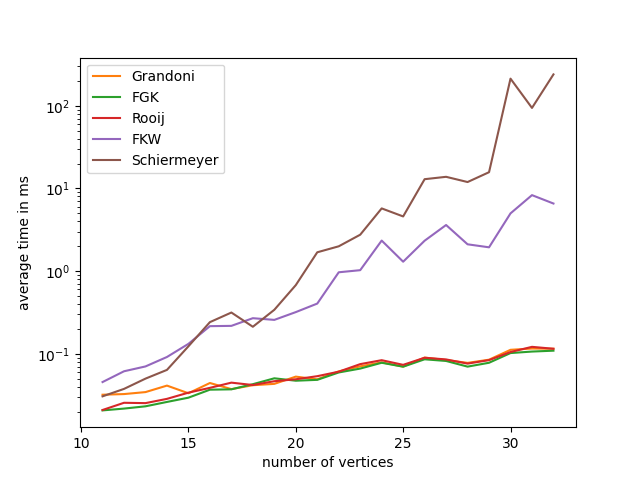
\includegraphics[width=0.9\textwidth]{figures/m3_average.png}
    \caption{average degree = 3}
    \label{fig:m3_average}
\end{figure}

\begin{figure}[H]
    \centering
    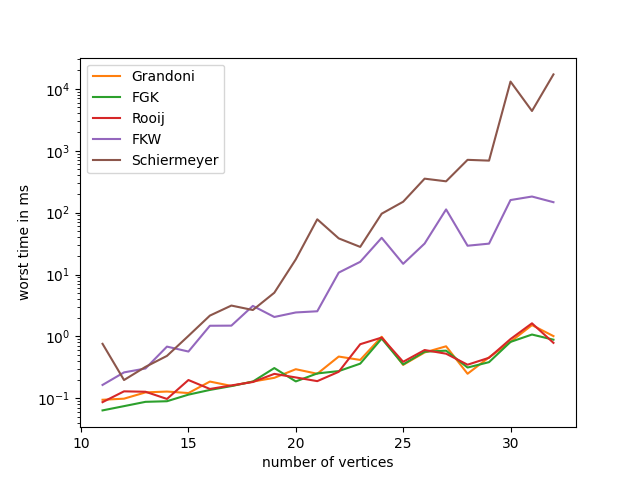
\includegraphics[width=0.9\textwidth]{figures/m3_worst.png}
    \caption{average degree = 3}
    \label{fig:m3_worst}
\end{figure}

\begin{figure}[H]
    \centering
    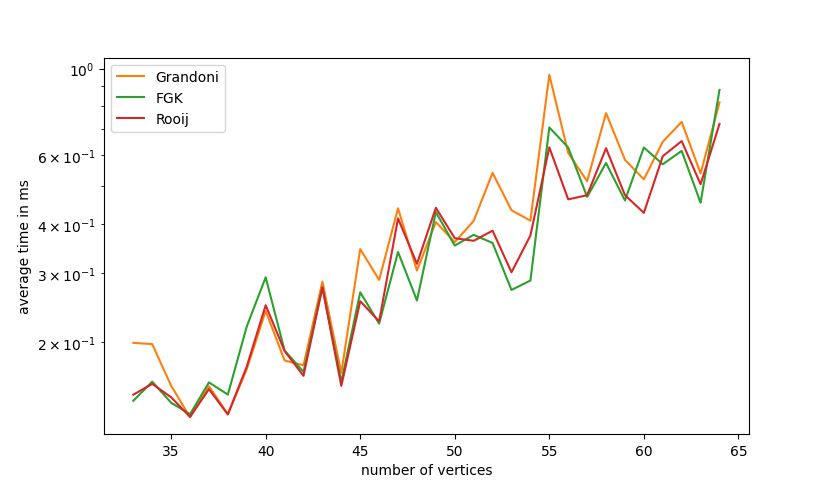
\includegraphics[width=0.9\textwidth]{figures/l3_average.png}
    \caption{average degree = 3}
    \label{fig:l3_average}
\end{figure}

\begin{figure}[H]
    \centering
    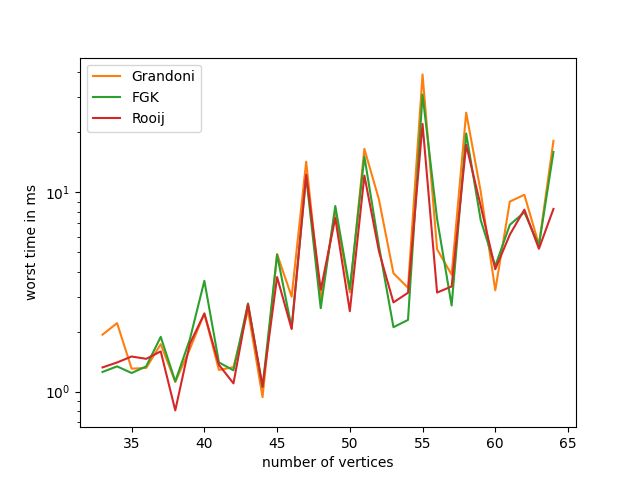
\includegraphics[width=0.9\textwidth]{figures/l3_worst.png}
    \caption{average degree = 3}
    \label{fig:l3_worst}
\end{figure}

\begin{figure}[H]
    \centering
    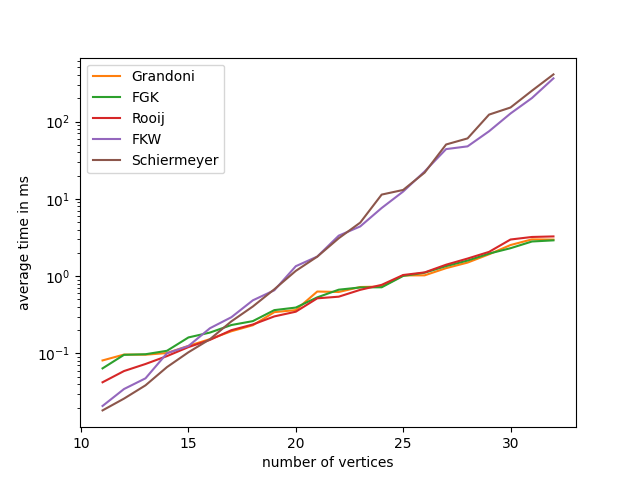
\includegraphics[width=0.9\textwidth]{figures/m6_average.png}
    \caption{average degree = 6}
    \label{fig:m6_average}
\end{figure}

\begin{figure}[H]
    \centering
    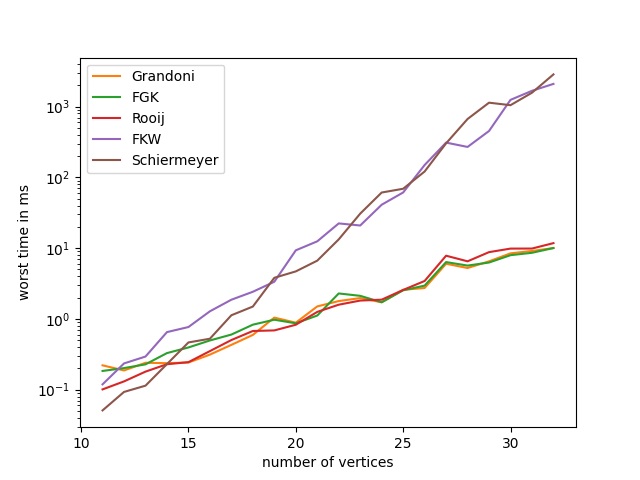
\includegraphics[width=0.9\textwidth]{figures/m6_worst.png}
    \caption{average degree = 6}
    \label{fig:m6_worst}
\end{figure}

\begin{figure}[H]
    \centering
    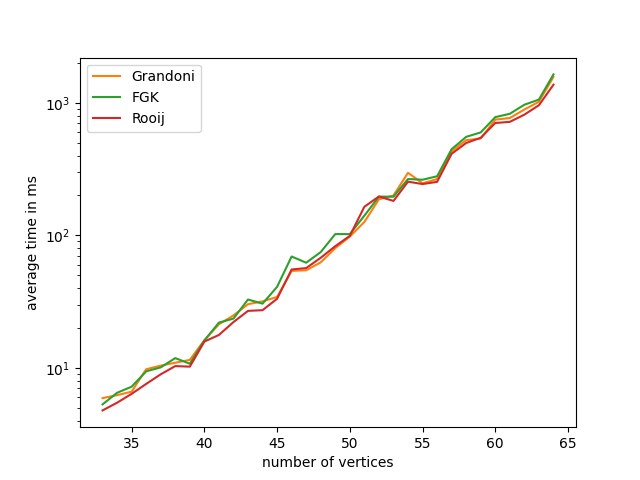
\includegraphics[width=0.9\textwidth]{figures/l6_average.png}
    \caption{average degree = 6}
    \label{fig:l6_average}
\end{figure}

\begin{figure}[H]
    \centering
    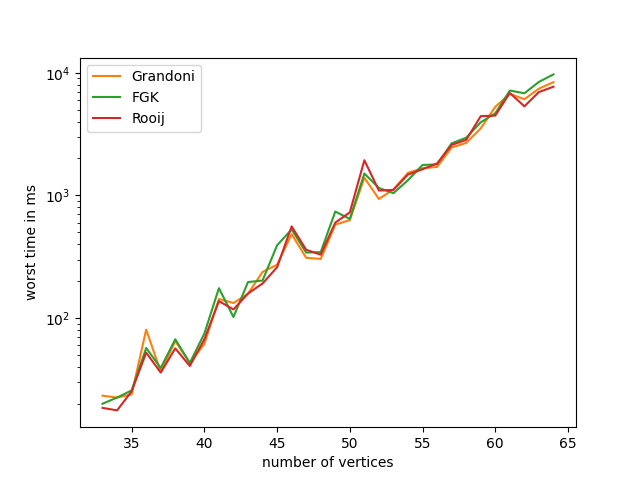
\includegraphics[width=0.9\textwidth]{figures/l6_worst.png}
    \caption{average degree = 6}
    \label{fig:l6_worst}
\end{figure}

\begin{figure}[H]
    \centering
    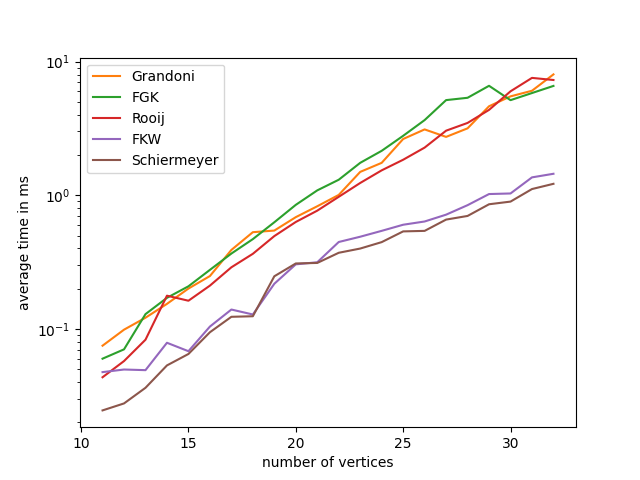
\includegraphics[width=0.9\textwidth]{figures/dense_average.png}
    \caption{average degree = $\frac{n-1}{2}$}
    \label{fig:dense_average}
\end{figure}

\begin{figure}[H]
    \centering
    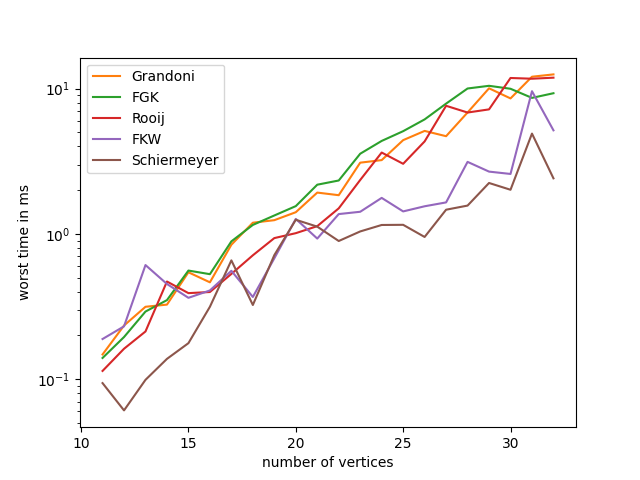
\includegraphics[width=0.9\textwidth]{figures/dense_worst.png}
    \caption{average degree = $\frac{n-1}{2}$}
    \label{fig:dense_worst}
\end{figure}

\begin{figure}[H]
    \centering
    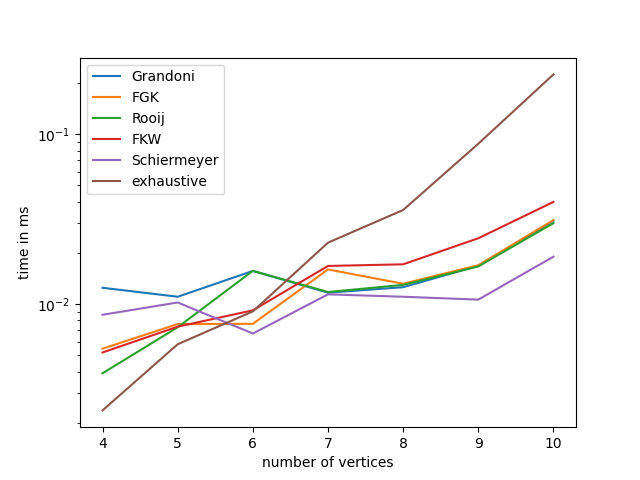
\includegraphics[width=0.9\textwidth]{figures/small_all_average.png}
    \caption{all graphs between 4 and 10 vertices, average time}
    \label{fig:small}
\end{figure}